\chapter{数据结构与算法}

\section{算法}

\subsection{算法(Algorithm)}

算法是一个很古老的概念,最早来自数学领域。 \\

有一个关于算法的小故事:在很久很久以前,曾经有一个顽皮又聪明的熊孩子,天天在课堂上调皮捣蛋。终于有一天,老师忍无可忍,对熊孩子说:

\begin{figure}[H]
	\centering
	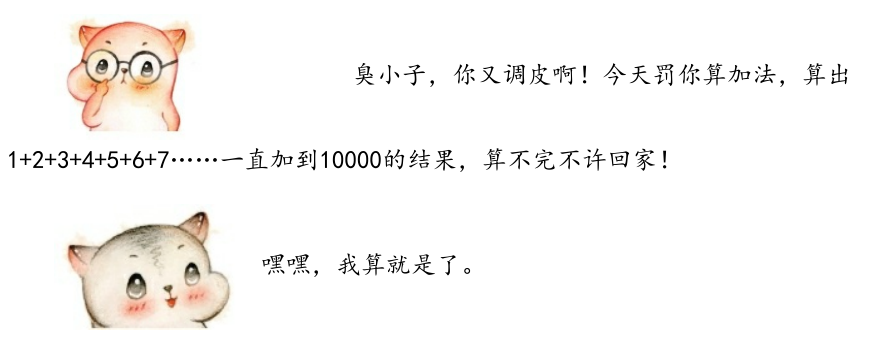
\includegraphics[scale=0.7]{img/C1/1-1/1.png}
\end{figure}

老师以为,熊孩子会按部就班地一步一步计算:

\vspace{-1cm}

\begin{align*}
	1 + 2  & = 3  \\
	3 + 3  & = 6  \\
	6 + 4  & = 10 \\
	10 + 5 & = 15 \\
	\dots
\end{align*}

这还不得算到明天天亮?够这小子受的!老师心里幸灾乐祸地想着。谁知仅仅几分钟后……

\begin{figure}[H]
	\centering
	
\includegraphics[scale=0.7]{img/C1/1-1/2.png}
\end{figure}

看着老师惊讶的表情,熊孩子微微一笑,讲出了他的计算方法。 \\

首先把从1到10000这10000个数字两两分组相加:

\vspace{-1cm}

\begin{align*}
	1 + 10000 & = 10001 \\
	2 + 9999  & = 10001 \\
	3 + 9998  & = 10001 \\
	4 + 9997  & = 10001 \\
	\dots
\end{align*}

一共有$ 10000 \div 2 = 5000 $组,所以1到10000相加的总和可以这样来计算:

$$
	(1 + 10000) \times 10000 \div 2 = 50005000
$$

这个熊孩子就是后来著名的犹太数学家约翰·卡尔·弗里德里希·高斯,而他所采用的这种等差数列求和的方法,被称为高斯算法。

\begin{figure}[H]
	\centering
	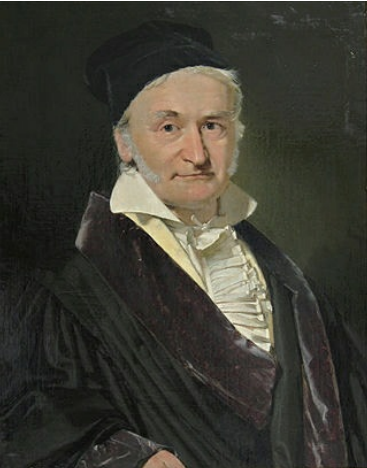
\includegraphics[scale=0.6]{img/C1/1-1/3.png}
	\caption{约翰·卡尔·弗里德里希·高斯}
\end{figure}

算法是解决问题的一种方法或一个过程,是一个由若干运算或指令组成的有穷序列。求解问题的算法可以看作是输入实例与输出之间的函数。 \\

算法有5个特点:

\begin{enumerate}
	\item 有穷性(finiteness):算法必须能在执行有限个步骤之后终止。
	\item 确定性(definiteness):算法的每一步骤必须有确切的定义。
	\item 输入项(input):一个算法有0个或多个输入。
	\item 输出项(output):一个算法有一个或多个输出,没有输出的算法是毫无意义的。
	\item 可行性(effectiveness):算法中执行的任何计算步骤都是可以被分解为基本的可执行的操作步。
\end{enumerate}

\subsection{算法描述}

算法是可完成特定任务的一系列步骤,算法的计算过程定义明确,通过一些值作为输入并产生一些值作为输出。 \\

流程图(flow chart)是算法的一种图形化表示方式,使用一组预定义的符号来说明如何执行特定任务。

\begin{itemize}
	\item 圆角矩形:开始和结束
	\item 矩形:数据处理
	\item 平行四边形:输入/输出
	\item 菱形:分支判断条件
	\item 流程线:步骤
\end{itemize}

\begin{figure}[H]
	\centering
	\begin{tikzpicture}[node distance=2cm]
		\node (start) [startend] {Start};
		\node (init)   [io, below of=start] {$ i = 0 $, $ sum = 0 $};
		\node (decision)  [decision, below of=init] {$ i \le 100 $?};
		\node (accumulation) [process, below of=decision] {$ sum = sum + i $};
		\node (update) [process, below of=accumulation] {$ i = i + 1 $};
		\node (output) [io, right of=decision, xshift=2.5cm] {print $ sum $};
		\node (end) [startend, below of=update] {End};

		\draw [arrow] (start) -- (init);
		\draw [arrow] (init) -- (decision);
		\draw [arrow] (decision) -- node[anchor=east] {yes } (accumulation);
		\draw [arrow] (accumulation) -- (update);
		\draw [arrow] (update) -- (-3,-8) -- (-3,-4) -- (decision);
		\draw [arrow] (decision) -- node[anchor=south] {no} (output);
		\draw [arrow] (output) |- (end);
	\end{tikzpicture}
	\caption{计算$ \sum_{i=1}^{100} i $的流程图}
\end{figure}

伪代码(pseudocode)是一种非正式的,类似于英语结构的,用于描述模块结构图的语言。使用伪代码的目的是使被描述的算法可以容易地以任何一种编程语言实现。